\documentclass{ximera}

\title{Section 3.4 Systems of Linear Equations}
\author{Conner Griffin}

\begin{document}
\begin{abstract}
    We solve systems of linear equations in two and three variables using elimination and substitution.
\end{abstract}
\maketitle

The set of solutions to the equation \(2x+4y =3\) form a straight line. There are few ways that we can express the solutions to this system. If we solve for \(y\) we get \(y = -\frac{1}{2}x + \frac{3}{4}.\) Then every solution as an order pair looks like \(\left(x, -\frac{1}{2}x + \frac{3}{4}\right).\) A graph of this line.

\desmos{b6wly9f2la}{100}{600}

What if we want all \((x,y)\) that satisfy two equations at once!

\begin{example}
    What do solutions to
    \[\begin{cases}
        2x+4y=3 \\
        -x+y =2
    \end{cases}\]
    look like?

    The following is a graph of solutions to both equations.

    \desmos{mnpol53mao}{100}{600}

    The only solution to both equations is the point of interesection for the two lines. In this case, \(\left(-5/6,7/6\right)\)
\end{example}

\begin{definition}
    A \emph{system of equations} is a finite collection of equations. A \emph{solution} to a system of equations in the variables \(x_1,x_2, \dots, x_n\) is an \(n\)-tuple \(\left(a_1,a_2, \dots, a_n\right)\) which is a solution to every equation in the system.
\end{definition}
\begin{example}The following is a general system of equations.
    \[\begin{cases}
        2x^{2}+y=2\\
        e^{x}+y=7
    \end{cases}\]
\end{example}
\begin{definition}
    A \emph{system of linear equations} is a finite collection of linear equations.
\end{definition}
\begin{example}
    The following are systems of linear equations.
    \[
    \begin{cases}
        2x+4y = 3 \\
        -x+y =2
    \end{cases}
    \]
    \[\begin{cases}
        \frac{1}{2}x + 3y -z =6 \\
        x+y+z=1 \\
        \sqrt{2}x - e y +7z
    \end{cases}\]
\end{example}
For a system of two linear equations in the variables \(x,y\) what can our set of solutions look like?

Our set of solutions can appear as the intersection of two arbitrary lines. We essentially have three scenarios. The system can be represented by two non-parallel lines. In such case, there is one unique solution. The system can be represent by two parallel, distinct lines. In this case, there are no solutions. The third situation, each equation is represented by the exact same line. In this case, the lines are still considered parallel; however, they are not distinct. There are infinitely many solutions.

\begin{image}
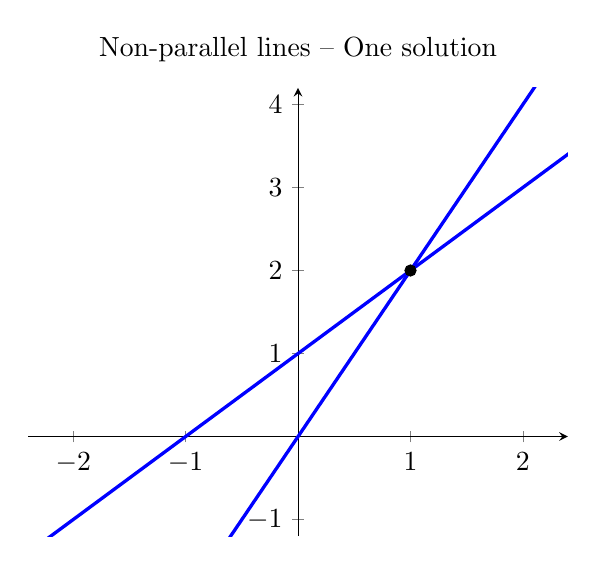
\begin{tikzpicture}
  \begin{axis}[
  title={Non-parallel lines -- One solution},
  xmin=-2.4,
  xmax=2.4,
  ymin=-1.2,
  ymax=4.2,
  axis lines=center,
  every axis y label/.style=
    {at=(current axis.above origin),anchor=south},
  every axis x label/.style=
    {at=(current axis.right of origin),anchor=west},
  ]
\addplot [very thick, blue, smooth, samples=100] {2*x};
\addplot [very thick, blue, smooth, samples=100] {x+1};
\addplot[mark=*] coordinates {(1,2)};
\end{axis}
\end{tikzpicture}
\end{image}
\begin{image}
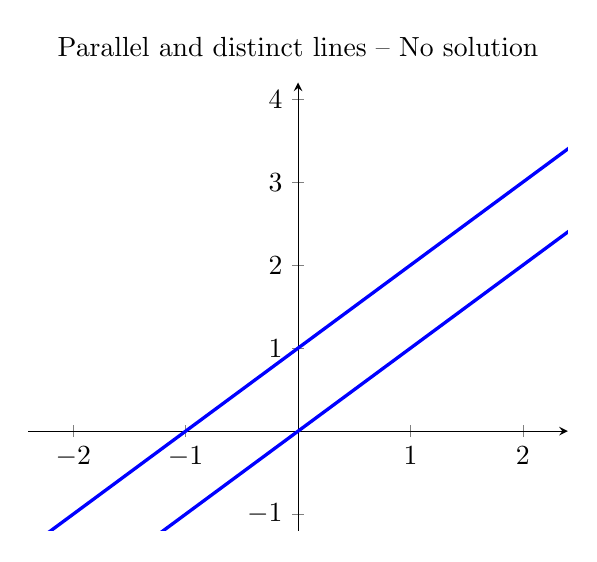
\begin{tikzpicture}
  \begin{axis}[
  title={Parallel and distinct lines -- No solution},
  xmin=-2.4,
  xmax=2.4,
  ymin=-1.2,
  ymax=4.2,
  axis lines=center,
  every axis y label/.style=
    {at=(current axis.above origin),anchor=south},
  every axis x label/.style=
    {at=(current axis.right of origin),anchor=west},
  ]
\addplot [very thick, blue, smooth, samples=100] {x+1};
\addplot [very thick, blue, smooth, samples=100] {x};
\end{axis}
\end{tikzpicture}
\end{image}
\begin{image}
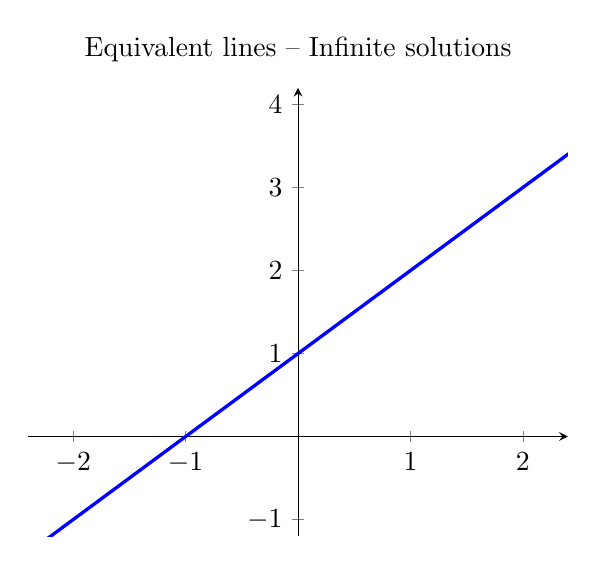
\begin{tikzpicture}
  \begin{axis}[
  title={Equivalent lines -- Infinite solutions},
  xmin=-2.4,
  xmax=2.4,
  ymin=-1.2,
  ymax=4.2,
  axis lines=center,
  every axis y label/.style=
    {at=(current axis.above origin),anchor=south},
  every axis x label/.style=
    {at=(current axis.right of origin),anchor=west},
  ]
\addplot [very thick, blue, smooth, samples=100] {x+1};
\end{axis}
\end{tikzpicture}
\end{image}
\begin{example}
    Let's solve the system
    \[\begin{cases}
        2x+4y =3 \\
        -x+y =2
    \end{cases}\]
    using one of the two methods we have, substitution.

    We first solve by substitution -- the best approach when dealing with only two equations and two unknowns.

    To solve a system by substitution, you will solve one equation for one of the variables and plug this expression into the other equation.

    Let's solve the bottom equation for \(y\) and plug this representation of \(y\) into the top equation.

    \[y = x+2 \rightarrow 2x+4\left(x+2\right) = 3.\]

    From this new equation in the single variable \(x,\) we can determine the \(x\) coordinate of the solution to the system of equations.

    \[2x+4\left(x+2\right) = 3 \rightarrow x = -\frac{5}{6}.\]

    We can plug this \(x\) into either of the other two equations to get the \(y\) coordinate of the solution.

    \[-\frac{5}{6} + 2 = \frac{7}{6}.\]

    The only solution to this system of equations is \(\left(-\frac{5}{6},\frac{7}{6}\right).\)
\end{example}

\begin{example}
    Let's solve the system
    \[\begin{cases}
        x+3y=9 \\
        \frac{1}{3}x+2y =2
    \end{cases}\]
    using the other of the two methods we have, elimination. The goal of this method is to ``eliminate'' variables from one of the equations. There are two things that we can do to the system that will not affect the system of equations. We can multiply an equation by any real number. This does not affect the set of solutions for the single equation and hence does not affect the set of solutions for the entire solutions. We can also add these scaled equations together. While this creates a new equations which has a different set of solutions, the set of solutions to both equations is preserved since these are the points at which we have equality.

    We will refer to \(x+3y=6\) as ``top'' and \(\frac{1}{3}x+y =2\) as ``bottom.'' We may eliminate the \(x\) from bottom by replacing bottom with \(-\frac{1}{3}top + bottom.\)

    \[\begin{matrix}
        &-x/3-y & = -3 \\
        + & x/3+2y & = 2 \\
        \hline & 0+y & =-1
    \end{matrix}\]

    Our new system.

    \[\begin{cases}
        x+3y=9 \\
        y =-1
    \end{cases}\]

    Now we can complete this problem by substituting \(y=-1\) into top; however, we continue with the elimination process.

    We now wish to eliminate \(y\) from the top equation. We accomplished this by replacing top with \(top-3bottom.\)

    \[\begin{matrix}
        &x+3y & =9 \\
        - &3y & =-3 \\
        \hline & x & = 12
    \end{matrix}\]

    Thus our solution is \(\left(12,-1\right).\)
\end{example}

We can solve a system with three variables and three unknowns with elimination, as well.
\end{document}